\section{Modularità}
L'obiettivo di questa sezione è di comprendere la differenza tra
\textbf{package}, \textbf{crate} e \textbf{moduli} e come organizzare un
progetto Rust mediante una \textbf{struttura gerarchica mantenibile}
controllandone la \textbf{visibilità} e \textbf{l'incapsulamento} delle
strutture dati.


\subsection{Perché rendere modulare un progetto?}

\begin{itemize}
  \item Per accrescere la \textbf{manutenibilità}: suddividere il
        codice in moduli rende più facile comprendere, modificare ed estendere
        nel tempo il progetto, riducendo il rischio di introdurre effetti
        collaterali non voluti
  \item Per favorire l'\textbf{incapsulamento}: controllando quali
        funzioni, tipi e campi siano esposti, pub, o tenuti privati. È possibile
        nascondere i dettagli implementativi ed assicurarsi che le altre
        parti del programma possano interagire solo con interfacce ben definite
  \item Per garantire una \textbf{sicurezza}, safety, all'atto della
        compilazione: il sistema di moduli e visibilità offerto da Rust permette
        di rilevare in fase di compilazione la maggior parte degli errori
        concettuali legati all'accesso ai dati, aumentando l'affidabilità del prodotto
  \item Per costruire librerie \textbf{riutilizzabili}: strutturare il
        codice in progetti, create, e moduli ben congegnati permette il riutilizzo
        di componenti, riducendo la duplicazione del codice e promuovendo
        l'uso consistente di funzionalità comuni
\end{itemize}


\section{Struttura di un progetto Rust: package, crate, moduli}

\begin{center}
  \begin{minipage}{\linewidth}
    % Primo blocco: 50% dello spazio per il codice
    \begin{minipage}{0.65\linewidth}
      Un progetto Rust è organizzato, chiamato, \textbf{package} eè
      rappresentato da una cartella con al suo interno un file \texttt{Cargo.
        toml} che gestisce la compilazione.


      Il package contiene la cartella \texttt{src} la quale contiene i
      vari \textbf{crate}. Se il package è semplice con un solo crate, il main,
      il quale verrà compilato aggiungendo, se necessario, i moduli aggiuntivi
      che abbiamo inserito. In questa maniera verrà creato un file eseguibile
      nella cartella \texttt{target/debug} con lo stesso nome del package.\newline


      Dentro questa cartella possono esserci più \textbf{crate}, la quale
      rappresenta l'unità di compilazione e può dare origine ad un eseguibile
      \texttt{main.rs} e/o ad una libreria \texttt{lib.rs}.\newline


      Il \textbf{modulo} è una suddivisione logica del codice, che può
      essere organizzata in file e cartelle. Organizza il codice e controlla la
      visibilità. Rappresenta lo spazio dei nomi all'interno di un crate.

    \end{minipage}% <-- IMPORTANTE: il simbolo % qui evita spazi bianchi extra
    \hfill
    \begin{minipage}{0.3\linewidth}

      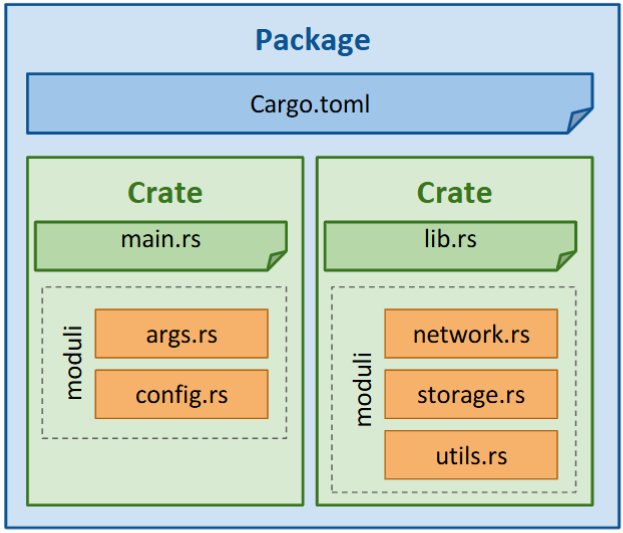
\includegraphics[width=\linewidth]{images/API_Programming/Moduli/M-esempio1.png}

    \end{minipage}
  \end{minipage}
\end{center}



% un profetto è chaiamto package, rappresetntao una cartella con il suo dentro il cargo.toml che gestisce la compilazione.

% dentro la cartella possono esserci più create, l'unnità di compilazione che il compilatore genererà una liberia o un binario (eseguibile)

% La cartellla del package contie la src nelle quali ci sono i vari crate, se è singolo 
% troviamo il main.rs. Questo file viene compilato lui a meno che non viene fa riferimento a moduli che vuole utilizzare (nel main troviamo mod nome_modulo) si tira dentro il modulo e poi lo compila.

% In questo modo ho creato un crate binario (in taget/debud mi trovo l'eseguibile chiamato come il nome del mio package).

% in src oltre al file main.rs posso trovare anche altri file, ad esempio lib.rs, verra compilato separatamente da main
% e conterrà i vari moduli. e in target/debug troveremo anche la liberiea. (libnome_package.rlib).

% La liberia può essere utilizzata dal main.

\section{Crates}

Il processo di compilazione di un progetto Rust è basato sul concetto di
\textbf{crate}. A livello sorgente, un crate è una unità di compilazione che ha
una radice, main.rs o lib.rs, e può essere composto da più moduli e file.
Un crate è l'unità di compilazione: Cargo compila ogni crate e poi li collega
tra loro.

% Ogni create di base è una unità di compilazione (con main.rs o lib.rs).
% I create binario che fanno capo a main.rs danno origine ad un eseguibile.


% Viceversa le liberie da un frammenot che può essere referenziato da altri exe divrsi, per condividere la funzionaliròà

% I create escono oltre che compialzione ma come versionemento e compionamento.
% Le liberire soo complse da compilare .
Un crate binario costituisce un'unità di versionamento e di caricamento in fase
di esecuzione. Quando un crate fa riferimento a codice, funzioni, strutture,
tratti, etc., esportato da un altro crate, di tipo libreria, quest'ultimo
deve essere combinato con il primo per mettere a disposizione quanto richiesto.
Questa operazione è detta di \textbf{linking} e dipende da come la libreria
è stata compilata, staticamente o dinamicamente.

% Il linking viene.

\begin{itemize}
  \item \textbf{Linking statico}: il codice della libreria viene incorporato
        direttamente nell'eseguibile durante la compilazione. Il risultato è un
        eseguibile più grande, ma indipendente da librerie esterne al momento
        dell'esecuzione.
  \item \textbf{Linking dinamico}: il codice presenta dei marcatori, stub, che
        indicano al sistema operativo di cercare la libreria dinamica (DLL su Windows,
        .so su Linux) al momento dell'esecuzione e di caricarla nello spazio del
        processo. Il risultato è un eseguibile più piccolo, ma dipendente dalla
        presenza della libreria dinamica al momento dell'esecuzione rendendone più
        difficile la distribuzione.
\end{itemize}
% Se la liberia è statica il linking viene a livello di compilazione.
% Se la libreria è dinamica nel .exe ci sono dei marcatori, staub, e il SO cerca la dll da mapparla nello spazio del processo.

% Sattico -> exe più grossi ma stabili
% dinamico -> exe più piccoli ma dipendenti da librerie esterne. Rende più difficilmente distributie .

Oltre a quanto detto fino ad ora, in Rust abbiamo la possibilità di versionare
il nostro crate. Nel file \texttt{Cargo.toml} è possibile specificarne la versione.

Oltre alla versione definita nel codice sorgente Rust, ogni progetto Cargo
espone la propria versione nel file \texttt{Cargo.toml}, seguendo il formato SemVer:

\begin{center}
  \begin{equation*}
    \text{version} = \text{"MAJOR.MINOR.PATCH"}
  \end{equation*}
\end{center}

% Oltre a queso in rust abbiamo la versione nel cargo.toml dove troviamo il version.
% Se cambio 0.1.2 -> 1.1.2 -> major chaneg (leggo i pdf e non più i csv)
% 0.1.2 -> 0.2.2 -> (oltre che ai csv leggo anche i pdf)
% 0.1.2 -> 0.1.3 -> (solo bug fix)
% majour.minou.patch

Le tre componenti hanno significati precisi:

\begin{itemize}
  \item \textbf{MAJOR}: viene incrementato quando si introducono breaking
        changes, cioè modifiche incompatibili con le versioni precedenti. Esempio: da
        0.1.2 a 1.1.2 se il programma smette di leggere CSV e inizia a leggere solo
        PDF.
  \item \textbf{MINOR}: viene incrementato quando si aggiungono nuove
        funzionalità retrocompatibili. Esempio: da 0.1.2 a 0.2.2 se, oltre ai CSV già
        supportati, il programma acquisisce la capacità di leggere anche i PDF.
  \item \textbf{PATCH}: viene incrementato quando si rilasciano sole correzioni
        di bug, senza aggiungere né rimuovere funzionalità. Esempio: da 0.1.2 a 0.1.3.
\end{itemize}

\section{Organizzazione del codice}

Spesso i package contengono due crate. Un create binario, facente capo a main.rs,
ed un crate libreria, facente capo a lib.rs. Questo permette di separare
l'interfaccia eseguibile dalla logica riutilizzabile del programma.

% La ragione per cui crediamo .exe e .lib è la fabilità con cui posso scrviere
% lib che possono essere condivise.

\subsection{Create binario}

Il main, minimale, si occupa solo dell'orchestrazione generale del programma come:
\begin{itemize}
  \item Parsing degli argomenti da linea di comando
  \item Configurazione dell'ambiente di esecuzione
  \item Chiamata alle funzioni della libreria per eseguire la logica
\end{itemize}
% Il main è minimale eg persing dei file eventualmente paragamtri di configurazion e
% chiamo le fuznion della liberia. 


\subsection{Le librerie}

Le librerie si occupano della logica dell'applicazione, funzioni, strutture dati,
moduli, etc., che può essere riutilizzata

\begin{itemize}
  \item Da più create binari dello stesso package
  \item Da altri progetti Rust
  \item Da altri linguaggi di programmazione, se esposte con interfacce
        compatibili (ad esempio, C)
\end{itemize}


% Nella liberia scrivo la logica della mia applicazione, può essere usarta oltre dal main che è li affiacno
% ma anche da altri .exe o anche dall' .exe del packege.

% Eg vector sta nella liberia standard std, file std::io

\subsection{Package con più file binari}



\begin{center}
  \begin{minipage}{\linewidth}
    % Primo blocco: 50% dello spazio per il codice
    \begin{minipage}{0.75\linewidth}
      Come abbiamo appena accennato un progetto può avere più file binari che utilizzano
      la stessa libreria. Se presenti essi devono essere collocati nella cartella
      \texttt{src/bin}.
      A questo punto il comando \texttt{cargo build} darà origine a più eseguibili.


      Questo permette di creare applicativi correlati, ad esempio un client e un server,
      che condividono dipendenze, hanno la stessa versione e vengono compilati insieme.


      \begin{tcolorbox}
        \textbf{Nota: }Un package è un contenitore di progetto che può includere uno
        o più crate binari, permettendo di sviluppare più programmi correlati che
        condividono codice comune.
      \end{tcolorbox}
    \end{minipage}% <-- IMPORTANTE: il simbolo % qui evita spazi bianchi extra
    \hfill
    \begin{minipage}{0.2\linewidth}

      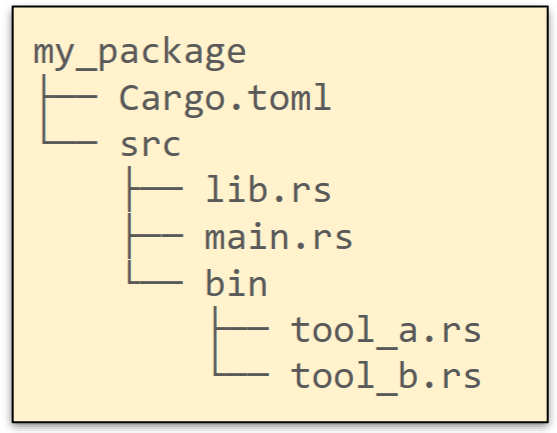
\includegraphics[width=\linewidth]{images/API_Programming/Moduli/M-esempio2.png}

    \end{minipage}
  \end{minipage}
\end{center}

% All'interno di una package oltre all'eseguibile principale possiamo avere altri eseguibili
% perché magrai produciamo ecosistemi eg appliczione di rete (client e server)
% I dati che si scambiano li incastro in una liberia comune.

% in src mettia una bin e i file che troviamo qui dentro sono interpretato come se fossero il main.
% danno origine

Un package è il contenitore del progetto. Può esporre una sola libreria, la lib.rs,
ma può dipendere da quante librerie esterne si vuole, dichiarandole come
dipendenze nel file Cargo.toml

% minted

% use pack1::hello
% fn main(){
%     print (questa è prsa da un aliberie hello())
%   }

% pack1 è il nome della cartella (il package)

% di base tutti gli eseguibili, il main e le lib possono contenter il loro codce
% e può diventare grandissimo ma noi vogliamo evitare >100 righe, 50 meglio perché poi
% non si leggono.
% la singola suddivisione è chiamata modulo, oltre che diveire il sorgere in file più picoli
% è anche la base della visibilità.
% dentro il singolo file sono visibile ed accessibili, fuoiri solo se cono marcate pub.

% Un modulo per diventare parte della compiazlione deves essere agganciato al suo contenitore.
% mod::cli il compilatore diventa parte della compilazione stessa.

% il modulo può dividersi in sottomoduli

\section{Moduli e visibilità}

Il codice contenuto in un crate è costituito da un albero di \textbf{moduli} che
oltre a dividere il sorgente in più piccoli, ne definisce anche la visibilità.
Un modulo è un costrutto sintattico, introdotto dalla parola chiave mod e dal
relativo nome che racchiude funzioni, tipi definiti dall'utente (struct, enum,
union), tratti, relative implementazioni ed altri moduli.

Tutto il codice che non è racchiuso in un modulo di tipo \textit{mod nome\_modulo{...}}
fa parte del modulo radice.

I moduli formano una gerarchia ad albero, la cui radice è l'unità di
compilazione corrente (rappresentata dalla parola chiave crate).

\subsection{Visibilità di default - privata}
Di base, tutti gli elementi definiti all'interno di un modulo sono considerati
privati, e sono accessibili solo al codice presente nel modulo stesso o nei suoi
sotto-moduli.

\subsection{Visibilità pubblica - pub}
Se un elemento definito all'interno di un modulo m1 è preceduto dalla parola
chiave pub, diventa pubblico e può essere utilizzato dal codice presente in un
modulo m2 che non sia un suo discendente, a condizione che tutti gli
antenati del modulo m1 siano a loro volta accessibili al modulo m2
(perché pubblici o perchè il modulo m2 è contenuto al loro interno).


% \begin{minted}[breaklines]{rust}
% mod my_mod {
%   fn private_fn() {} // visibile solo nel modulo corrente
%   pub fn public_fn() {} // visibile nel contesto dell’unità di compilazione:
%                         // - codice presente in questo stesso file
%                         // - codice che ha accesso al percorso my_mod;
%   mod private_nested_mod { // sotto-modulo privato
%     fn test() {} // può accedere a my_mod::private_fn()
%   }
%   pub mod public_nested_mod { //accessibile a chi ha accesso a my_mod
%     pub fn api() {}
%   }
% }
% \end{minted}


% fn main() {
%     my_mod::public_fn();
%     my_mod::public_nested_mod::api();
%   }

\begin{center}
  \begin{minipage}{\linewidth}
    \begin{minipage}{0.55\linewidth}
      \begin{minted}[breaklines]{rust}
mod my_mod {
  fn private_fn() {} // visibile solo nel modulo corrente
  pub fn public_fn() {} // visibile nel contesto dell’unità di compilazione:
  // - codice presente in questo stesso file
  // - codice che ha accesso al percorso my_mod;
  mod private_nested_mod { // sotto-modulo privato
    fn test() {} // può accedere a my_mod::private_fn()
  }
  pub mod public_nested_mod { //accessibile a chi ha accesso a my_mod
    pub fn api() {}
  }
}
\end{minted}

    \end{minipage}
    \hfill%
    \begin{minipage}{0.4\linewidth}
      \begin{minted}[breaklines]{rust}

fn main() {
  my_mod::public_fn();
  my_mod::public_nested_mod::api();
}
\end{minted}

      \vspace{0.5cm}

      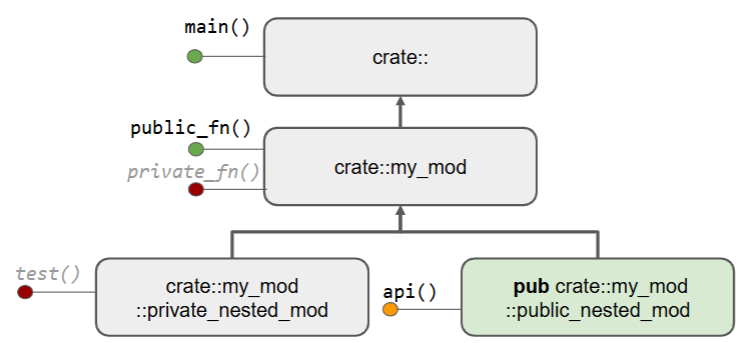
\includegraphics[width=1\linewidth]{images/API_Programming/Moduli/M-esempio3.png}

    \end{minipage}

  \end{minipage}
\end{center}

Per poter usare un simbolo (funzione, tipo, tratto, etc. ) definito in un
modulo diverso da quello corrente occorre indicare al compilatore dove andare a
reperirlo.

Lo si può fare indicando il path del modulo. Questo path può essere
assoluto o relativo.

\subsection{Cammino assoluto}
Il cammino assoluto comincia con il nome del create in cui si trova il simbolo
seguito dalla sequenza gerarchica di di moduli che occorre attraversare per
giungere al simbolo.

\begin{center}
  \mintinline{rust}{let size = std::mem::size_of::<i32>(&f);}
\end{center}

si utilizza il separatore \textbf{::} per connettere i nomi dei (sotto-)moduli.

% per usare un simbolo di qualche tipo in un modulo diversio lo devo indicare con tutto il nome
% Nome assoluto crate:: o std:: se è la liberia esterna

Nel caso il simbolo appartenga al crate corrente, si può indicare come elemento
iniziale la parola chiave \textbf{crate}.

\subsection{Cammino relativo}
Il cammino relativo comincia con le parole chiave \textbf{self} o \textbf{super}.
Un parallelismo potrebbe essere, in ordine, il concetto di "./" e "../" nei file
system.

\begin{center}
  \mintinline{rust}{self::my_function}\\
  \mintinline{rust}{super::my_function}
\end{center}

% quadno uso rieriemnti relativi (eg../ o ./ nei file) lo faccio con self (./) o
% super (../)

\subsection{Cammino e *}

Per evitare di dover ripetere l'intero cammino per ogni occorrenza del simbolo,
è possibile usare il costrutto.

\begin{center}
  \mintinline{rust}{use path::del::modulo::*;}
\end{center}

Questo rende disponibile, nel file corrente, la definizione di tutti i simboli
pubblici del modulo indicato.

% con * porto dentro tutto quello del pubblic nei moduli. non una grande idea,
% perché se il nome è uguale colide con quello nostro o di altre librerie.
% meglio usare solo i simbolo che servono davvero

Per poter accedere ad un simbolo occorre che tutti gli elementi del cammino
siano accessibili a chi ne fa richiesta, ovvero essere dichiarati come pubblici
o contenere il modulo corrente.\newline

Un modulo può esportare tutti i simboli pubblici di un proprio sottomodulo come
fossero propri con il costrutto \mintinline{rust}{pub use submodule::*;}.
Questo facilita la costruzione di librerie in cui viene semplificata l'API
pubblica, nascondendo i dettagli della struttura interna.

Inoltre facilita l'evoluzione del codice, permettendo di modificare la struttura
interna dei moduli senza modificare il codice che dipende da essi, mantenendo
invariata l'interfaccia pubblica.

% inoltre è possibile pub use submodule::*; ovvero tutti i simboli pubblici 
% del sottomodulo rendili visibile come se fossero esportati da me.nascondendo 
% che vengono da altre libr
% perch?
% 1. non complicare la vita a chi usa la mia liberia, nascondendo compelssità
% 2. facilità di evoluzione del mio codice, prima prendevo beta dalla liberia ma se la voglio combiare non includo più qella liberia ma uso quella mia che ho appena scritto, nel caso torno indietro.


\section{Moduli e file sorgente}

Il codice relativo ad un sotto-modulo può essere inserito:

\begin{itemize}
  \item Nello stesso file sorgente del modulo genitore, con la notazione
        \mintinline{rust}{mod nome_modulo{...}}
  \item In un file sorgente a sé, presente nella stessa cartella, chiamato
        \texttt{nome\_modulo.rs}, in questo caso occorre che il modulo genitore sia
        presente la dichiarazione del modulo, nel formato \mintinline{rust}{mod nome_modulo;}
  \item Nella sotto-cartella chiamata \texttt{nome\_modulo} possono essere
        collocati i file sorgente di eventuali sotto-moduli di \texttt{nome\_modulo}
\end{itemize}


% spesso il sottomodulo è in un file e nel geneitro mettiamo mod nome_modulo.


% può essere che il sottomodulo debba essere suddiviso in sottosottomoduli e li mettimao
% dentro una cartella con lo stesso nome del sottomodulo.

% mod::utils nel main

Eventuali crate esterni, non facenti parte della gerarchia di moduli definiti
dal package corrente, vengono elencati nel file cargo.toml che descrive la
struttura del package stesso.

Nella sezione [dependencies] sono presenti, uno
per riga, i nomi dei crate da importare con l'indicazione della relativa
versione


\begin{center}
  \begin{minipage}{\linewidth}
    % Aggiunto [t] qui sotto
    \begin{minipage}[t]{0.48\linewidth}
      \subsection{Struttura di un progetto eseguibile Rust}
      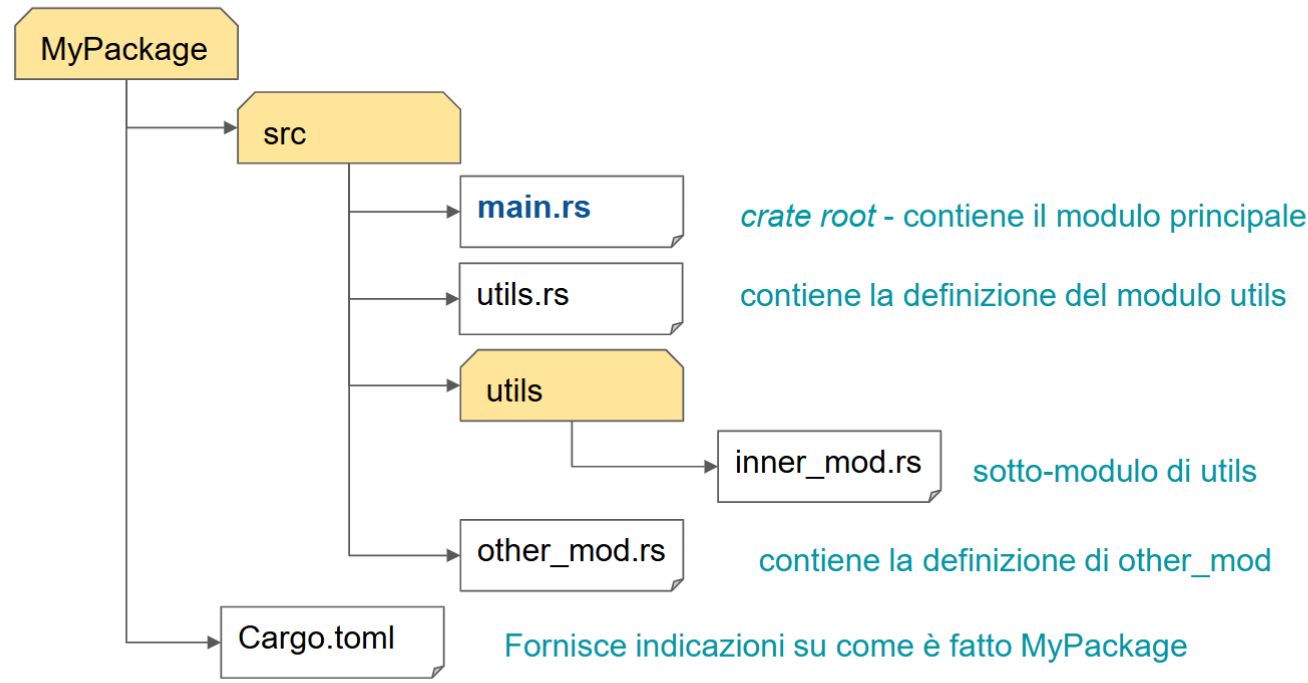
\includegraphics[width=1\linewidth]{images/API_Programming/Moduli/M-esempio4.png}
    \end{minipage}
    \hfill%
    % Aggiunto [t] qui sotto
    \begin{minipage}[t]{0.48\linewidth}
      \subsection{Struttura di un progetto con due o più eseguibili}
      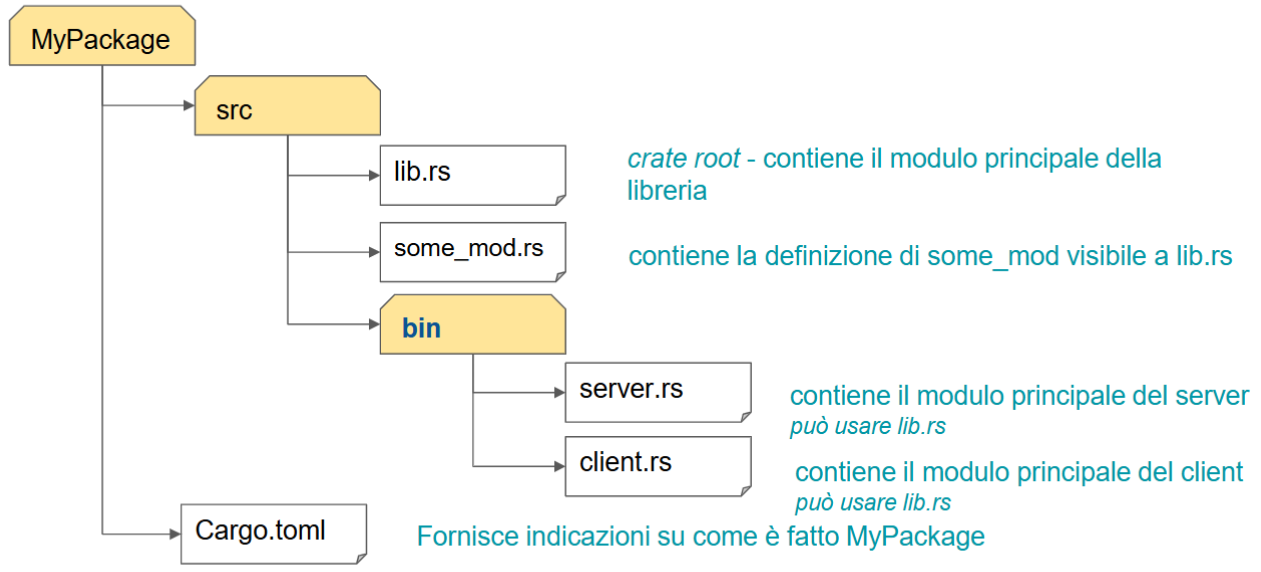
\includegraphics[width=1\linewidth]{images/API_Programming/Moduli/M-esempio5.png}
    \end{minipage}
  \end{minipage}
\end{center}


\section{Librerie}
% Una liberia la usaiamo non per avere un eseguibile ma per avere un insie di fuznio da utilizzare da altri programmi
% concetto di:

Una libreria è un crate che non produce un programma eseguibile, ma fornisce
funzionalità riutilizzabili sotto forma di funzioni, strutture dati, tratti e
moduli che possono essere utilizzati da altri crate.

Le librerie permettono di:

\begin{itemize}
  \item \textbf{Riutilizzare} codice in più programmi
  \item \textbf{Separare} la logica dell'applicazione dall'interfaccia eseguibile
  \item \textbf{Organizzare} meglio progetti complessi
  \item \textbf{Condividere} funzionalità tra progetti con linguaggi diversi
\end{itemize}


% risuso
% concetto di separazione
% condivsione con altri linuaggi di compialzione (rust velocità e python facilità di mettere su un pgm) grazie all'isolamnto

Una libreria espone una API (Application Programming Interface), cioè un insieme
di elementi pubblici che possono essere utilizzati dall'esterno.
Gli elementi pub fanno parte dell'API, mentre gli elementi privati sono dettagli
di implementazione.

\section{Librerie interne ed esterne}

Le librerie possono essere interne al package o esterne ad esso.

\begin{tcolorbox}
  \textbf{Nota: }Un package può contenere una sola libreria interna (src/lib.rs),
  ma fare riferimento a molte librerie esterne
\end{tcolorbox}

% di base la liberie che rust può usare sono quelle intere o esterne basta nel cargo.toml aggiungere il nome liberie e versione e l'ambiente cargo se la scarca.
% mi scarico ad un registry pubblico (crates.io) e scarco.

Le librerie esterne sono elencate nella sezione [dependencies] del file Cargo.toml.
Ciascuna riga indica il nome della libreria, la versione desiderata ed eventuali
opzioni di configurazione.
All'atto della costruzione di un progetto, le librerie esterne vengono
automaticamente scaricate dal sito https://www.crates.io e compilate a partire
dai loro sorgenti.
Solo dopo che tutte le dipendenze sono state compilate viene compilato il crate
dell'applicazione.


Una libreria esterna viene ricompilata solo se necessario, ad esempio quando:

\begin{itemize}
  \item Cambia la versione della dipendenza
  \item Cambiano le opzioni di compilazione
  \item Cambia il target o il profilo di build (debug / release)
\end{itemize}


% \subsection{Librerie ed interoperabilità}

% Le librerie permettono a programmi scritti in linguaggi diversi di utilizzare lo
% stesso codice compilato. In Rust è possibile creare librerie compatibili con
% altri linguaggi, ad esempio C, C++ o Python, esportando funzioni con
% un'interfaccia compatibile.

% Meccanismo di funzionamento:

% \begin{itemize}
%   \item Il codice Rust viene compilato come libreria condivisa o statica
%   \item Le funzioni esportate seguono la convenzione di chiamata C (ABI)
%   \item Programmi scritti in altri linguaggi possono caricare e invocare queste funzioni
% \end{itemize}


% Le liberie possono esere costrutte per un collegameto statico o dimanico.
% ovvero il linking (rimepimento dei buchi di codice) avvieen durante la compilazione e creazione del .exe
% oppure a caricameento dinamico (in fase di linking ) viene messo una stub e quando il pgm parte vai a cercare la libereia x e tirala dentro.



\subsection{Librerie ed interoperabilità}
Le librerie permettono a programmi scritti in linguaggi diversi di riutilizzare
lo stesso codice compilato. In Rust è possibile creare librerie compatibili con
altri linguaggi, come C, C++ o Python, esportando funzioni tramite
un'interfaccia compatibile con l'ABI del C.

Il meccanismo funziona come segue:
\begin{itemize}
  \item Il codice Rust viene compilato come libreria condivisa (\texttt{.so}/\texttt{.dll})
        o statica (\texttt{.a}/\texttt{.lib})
  \item Le funzioni esportate seguono la convenzione di chiamata C (\textit{C ABI})
  \item Programmi scritti in altri linguaggi possono caricare e invocare queste funzioni
\end{itemize}

Una libreria può essere collegata in due modalità:
\begin{itemize}
  \item \textbf{Linking statico} — il codice della libreria viene incorporato
        direttamente nell'eseguibile durante la compilazione. Il risultato è un
        singolo \texttt{.exe} autosufficiente, ma di dimensioni maggiori.
  \item \textbf{Linking dinamico} — durante la compilazione viene inserito un
        riferimento (\textit{stub}) alla libreria esterna. Al momento
        dell'avvio del programma, linking, il sistema operativo individua e carica in
        memoria la libreria richiesta (\texttt{.so} o \texttt{.dll}).
\end{itemize}


% In rust quando creiamo una lib possiamo definirla nel toml se la vogliamo statica o dinamica.
% inoltre cargo possiamo dire, chiamata anche libebrie fatte per il C o solo per rust.
% (il C è il defacto standar per le liberie).

Le applicazioni tipiche sono:

\begin{itemize}
  \item Usare Rust come motore ad alte prestazioni per componenti critici
  \item Integrare Rust in software esistente scritto in C/C++
  \item Creare binding per linguaggi di scripting come Python o JavaScript
\end{itemize}

\begin{figure}[htbp]
  \centering
  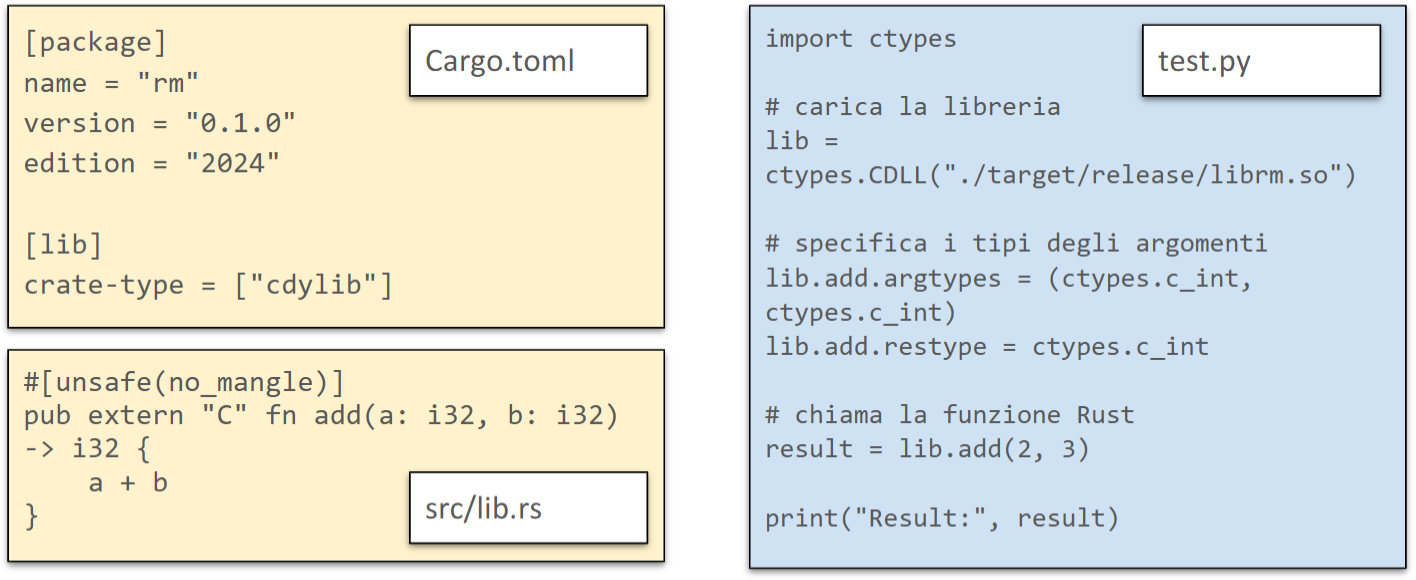
\includegraphics[width=0.6\textwidth]{images/API_Programming/Moduli/M-esempio6.png}
\end{figure}

\begin{tcolorbox}
  \textbf{Nota: } \texttt{\#[no\_mangle]} dice al compilatore Rust
  di non modificare il nome della funzione durante la compilazione, rendendola
  così accessibile da altri linguaggi con il nome esatto specificato nel codice
  sorgente. Senza questo attributo, il compilatore applica il name mangling, una
  tecnica che trasforma i nomi delle funzioni includendo informazioni aggiuntive
  come il percorso del modulo e un hash univoco, producendo nomi come
  \texttt{\_ZN7mycrate3add17h3f6a1c2b8e4d5f9eE}, illeggibili e non invocabili
  direttamente da altri linguaggi.
\end{tcolorbox}

% mangle:suggeriemnto per rust addi32i32 che sono i parametnti
% no\_mangle non mi interessa voglio eseguila su altri linguaggi e voglio solo che sia chiami add

% Vec non dobbiamo importarlo perché il compilatore li vede in autimantico tutte le cose nel prelude file

\section{Collegamento delle librerie}
La sezione [lib] del file Cargo.toml che descrive il progetto contiene dettagli
relativi al tipo di libreria che si intende creare. La chiave \textbf{crate-type}
può assumere i seguenti valori:


\begin{itemize}
  \item \textbf{rlib}: libreria statica Rust, valore di default,
        il file risultante può solo essere usato da altri eseguibili Rust che ne
        includeranno le parti importate direttamente nel proprio codice binario
  \item
        \textbf{dylib}: libreria dinamica Rust; viene trasformata in un file .dll in
        windows, .so in linux, .dylib in macOS; può essere utilizzata solo da codice
        Rust, ma sarà caricata in fase di esecuzione
  \item \textbf{cdylib}: libreria
        dinamica conforme alle specifiche C; viene trasformata in un file .dll in
        windows, .so in linux, .dylib in macOS; può essere usata da eseguibili scritti
        in altri linguaggi; se viene usata da un programma Rust deve essere inclusa
        sotto forma di funzioni esterne
  \item \textbf{staticlib}: libreria statica
        conforme alle specifiche C; viene trasformata in un file .lib in windows e .a in
        linux e macOS; può essere usata da eseguibili scritti in altri linguaggi; se
        viene usata da un programma Rust deve essere inclusa sotto forma di funzioni
        esterne
\end{itemize}

\section{Preludio}

Come in molti linguaggi di programmazione, anche in Rust esiste un insieme di
simboli, funzioni, tipi e tratti, come Vec e String, che sono sempre disponibili 
in ogni modulo senza includere esplicitamente alcuna dichiarazione anche se facenti 
parte di create diversi dal crate corrente.

Questi sono elencati all'interno di un modulo chiamato \mintinline{rust}{std::prelude} 
che viene importato automaticamente all'atto della compilazione di un file sorgente.
In questo modo si evita di rendere verboso il codice sorgente.


Ogni versione di Rust viene con un proprio preludio. Cargo provvede ad
includere quello corretto in funzione del valore dell'attributo package/edition
nel file Cargo.toml.


\section{Clap - libreria per la gestione dei parametri da linea di comando}

La libreria clap gestisce in modo dichiarativo i parametri passati attraverso la
linea di comando.

La si include in un crate aggiungendo, nel file Cargo.toml, questa dipendenza:

\begin{minted}{rust}
[dependencies]
clap = { version = "4.5", features = ["derive"] }
\end{minted}


Questo mette a disposizione un insieme di macro e di strutture dati che
permettono di descrivere una struttura dati in cui verranno depositati i valori
estratti dalla riga di comando, così come di derivare automaticamente una
funzione di analisi che provvede a valorizzare i campi di tale struttura.

Questa libreria permette anche di esprimere programmaticamente l'insieme dei
parametri, la tipologia di valori associati e gli eventuali vincoli associati, basata
sul pattern builder.


\begin{center}
  \begin{minipage}{\linewidth}
    % Aggiunto [t] qui sotto
    \begin{minipage}[t]{0.44\linewidth}
      
\begin{minted}[breaklines]{rust}
use clap::Parser;
/// Simple program to greet a person
#[derive(Parser, Debug)]
#[command(version, long_about = None)]
struct Args {
  /// Name of the person to greet
  #[arg(short, long)]
  name: String,
  /// Number of times to greet
  #[arg(short, long, default_value_t = 1)]
  count: u8,
}

fn main() {
  let args = Args::parse();
  for _ in 0..args.count {
    println!("Hello {}!", args.name)
  }
}
\end{minted}

    \end{minipage}
    \hfill%
    % Aggiunto [t] qui sotto
    \begin{minipage}[t]{0.54\linewidth}
\begin{minted}[breaklines]{rust}
$ demo --help
Simple program to greet a person

Usage: demo[EXE] [OPTIONS] --name <NAME>

Options:
-n, --name <NAME> Name of the person to greet
-c, --count <COUNT> Number of times to greet [default: 1]
-h, --help Print help
-V, --version Print version

$ demo --name Me
Hello Me!
\end{minted}

    \end{minipage}
  \end{minipage}
\end{center}
